
\section{System Model}
\label{sec:model}

In this section, we present our model for transactions, invariants,
and coordination.

\minihead{Databases and Transactions} In this paper, we consider a set
of users accessing a shared database, which contains a
\textit{versioned} set of data items. In our initial formulation, we
will represent database state as a bag of mutations (much like a
write-ahead log~\cite{gray-book}), but we will consider other, more
pragmatic representations in Section~\ref{sec:bcc-practice}; we assume
that the database is initially populated by an initial state $D_0$
(typically but not necessarily empty). Copies of database state can be
combined via a ``merge'' operator ($\sqcup$: $DB \times DB \rightarrow
DB$). In our ``bag of mutations'' model, merge is simple set union,
but we will consider alternative implementations in
Section~\ref{sec:bcc-practice}.

Users submit requests to the database in the form of transactions, or
groups of operations on data items that should be executed together:
we define a transaction $T$ as a transformation on state: $T: DB
\rightarrow DB$. Individual operations are often in the form of writes
(which add new versions to the database) or reads (which return a
specific set of versions from the database), but operations can also
operate on abstract data types, such as incrementing a counter item or
adding an item to a set item. When required---and certainly in later
sections of this paper---we will discuss specific operation types,
but, in general, we will not make any specific assumptions about
operations. A transaction can \textit{commit}, signaling success, or
\textit{abort}, signaling failure. As a pragmatic guarantee (though
not strictly required for our results), we will not consider versions
produced by aborted transactions in our analysis (i.e., Read Committed
isolation, achievable by waiting to include versions until commit
time~\cite{hat-vldb,spanner}), and, if a transaction commits, its
effects should survive database failures (i.e., transactions should be
durable).

\minihead{Invariants} As we have discussed, users accessing a shared
database have notions of correctness, which we capture in our system
model via \textit{invariants}. In our model, users specify invariants
over arbitrary database state that determine whether a given state is
valid according to application rules. We model invariants as binary
predicates on database state: $I: DB \rightarrow \{true,
false\}$. Given a set of invariants $I_s$, we say that the database is
\textit{valid} under $I_s$ if all invariants in $I_s$ evaluate to
true; we also require that $D_0$ be valid. For example, an invariant
might express the requirement that only one user in a database has a
given ID. Invariants directly capture the notion of ACID
Consistency~\cite{bernstein-book,gray-virtues}.

\miniheadnostop{Why specify invariants?} Much of the existing work on
database concurrency control assumes a model whereby ``the [set of
  invariants] is generally not known to the system but is embodied in
the structure of the transaction''~\cite{traiger-tods}. Indeed,
Eswaran et al.'s seminal paper on the topic of consistency argues that
``a complete set of assertions would no doubt be as large as the
system itself''~\cite{eswaran-consistency}. Nevertheless, since 1976,
databases have introduced support for a finite set of
invariants~\cite{korth-serializability} in the form of primary key and
foreign key, uniqueness, and row-level ``check'' constraints. We
expand this set of invariants in Section~\ref{sec:bcc-practice} and
demonstrate that a small set of invariants provides expressive power
for many applications. It is possible to perform a conservative
analysis if a complete specification of invariants is missing, but
this will result in less useful results. Unlike more general forms of
axiomatic logic (e.g., Hoare-style triples~\cite{decomp-semantics}),
we require only one set of invariants per application.\vspace{.5em}

\minihead{Coordination} In this paper, we are concerned with
synchronization and coordination between multiple transactions. To
begin, we consider a system model with replicated copies of database
state (\textit{replicas}) located in separate processes
(\textit{servers}) that can each respond to transaction requests.  To
prevent the system from unnecessarily aborting transactions in order
to provide a response, we say that a system provides
\textit{transactional availability} (liveness) if, whenever a client
executing a transaction $T$ can access at least one replica for each
item in $T$, $T$ eventually commits or otherwise aborts itself either
due to an \textit{abort} operation in $T$ or due to a violation of a
declared integrity constraint~\cite{hat-vldb}.\footnote{As Bailis et
  al. note~\cite{hat-vldb}, this definition precludes multi-server
  fault tolerance (durability). However, we can consider multi-server
  durability by extending this definition to include coordination with
  a (typically small~\cite{bigtable,spanner,dynamo}) fixed number of
  servers. This does not greatly affect scalability because, as more
  replicas are added, durability-related communication is constant.}
We say that a system is \textit{always valid} if all replicas always
observe valid state. To capture the effect of network partitions but
also to capture linear scalability, we say that a system is
\textit{\cfree} if replicas do not communicate in order to execute
transactions.

It is vacuously possible to maintain ``consistent'' database states by
letting replicas diverge: in distributed systems parlance, this
guarantees \textit{safety} but not
\textit{liveness}~\cite{lamport-safety}. To ensure that replicas
eventually agree---reflecting a shared, common set of database
state---we will say that a system is \textit{convergent} if, in the
absence of new transactions and in the absence of indefinite
communication delays, all replicas eventually contain the same state
(i.e., via \textit{anti-entropy} processes)~\cite{vogels-defs}. To
capture the process of reconciling divergent copies of database state,
we introduce a \textit{merge} operator (denoted $\sqcup$) that, given
two copies of divergent database state, reconciles them by producing a
single copy of database state. For our initial presentation, our merge
operator will be simple set union, but we discuss alternative merge
operators in Section~\ref{sec:merge}. We make no assumptions about
merge except that it be commutative, associative, and
idempotent~\cite{calm,crdt}. Importantly, to provide convergence, this
merge operator will be applied \textit{asynchronously} and can safely
stall at any point given that---at some point in the future---merging
occurs.

Figure~\ref{fig:replicas} depicts a coordination-free execution of two
transactions $T_1$ and $T_2$ on two separate replicas of (complete)
database state. Each transaction commits on its local replica, which
subsequently forwards the new database state to the other replica in
the background. By applying the merge operator of set union, each
replica contains the same database state.

\begin{figure}
\begin{center}
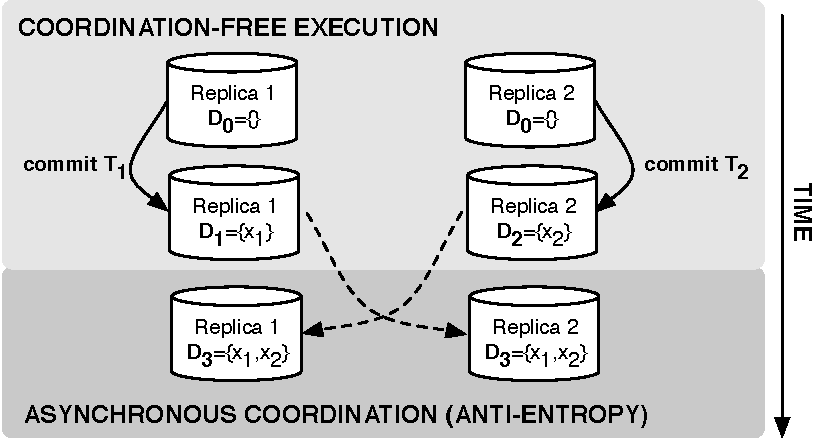
\includegraphics[width=.85\columnwidth]{figs/replicas.pdf}
\end{center}\vspace{-1em}
\caption{An example coordination-free execution of two transactions,
  $T_1$ and $T_2$ on two replicas of database state. Each transaction
  commits on a replica, then, after commit, the replicas exchange
  their new writes asynchronously and converge on a common database
  state ($D_3$).}
\label{fig:replicas}
\end{figure}

\miniheadnostop{Physical and logical replicas} While most treatments
of database systems treat replicas as individual servers, a
single-site database can also provide users with an interface that
exposes multiple ``replicas''. In fact, a multi-versioned database
system~\cite{bernstein-book} effectively provides each user with a
logical replica of database state that is isolated from concurrent
access and modification. A set of invariants and stored procedures
that are achievable without coordination in a distributed context can
also be executed in parallel on a single-site system without stalling
due to concurrent operations.  In fact, our current prototype
transaction model (Section~\ref{sec:evaluation}) is based on
multi-versioning and snapshot reads (``logical replicas'') rather than
physical multi-master replication.
